\capitulo{1}{Introducción}

El análisis del desarrollo de las estructuras craneales fetales es fundamental para la detección precoz de anomalías del sistema nervioso central. Entre estas estructuras, el cerebelo juega un papel clave, no solo en funciones motoras, sino también en el desarrollo cognitivo, emocional y del lenguaje. Durante el periodo de gestación, el cerebelo del feto experimenta una rápida expansión y crecimiento, especialmente entre las semanas 24 y 40, convirtiéndose en una región crítica para el estudio del neurodesarrollo fetal \cite{volpe2009}. 

Factores como la exposición materna al tabaco, al alcohol o ciertas toxinas ambientales pueden afectar negativamente al desarrollo del cerebelo, pudiendo derivar en un mayor riesgo de discapacidades neurológicas en la infancia \cite{koning2017impacts}. En este contexto, la evaluación objetiva del cerebelo fetal cobra una especial relevancia en el ámbito del diagnóstico prenatal.

Sin embargo, se trata de una tarea que requiere un alto nivel de experiencia, y en la que pueden surgir ligeras discrepancias interobservador debido a factores como la calidad de imagen, la variabilidad anatómica o las diferencias en los criterios de evaluación, lo que puede dificultar la estandarización del diagnóstico. 

En los últimos años, las técnicas de segmentación automática de imágenes han emergido como una herramienta prometedora para superar estas limitaciones \cite{hesamian2019}. Aplicadas al plano transcerebeloso, estas técnicas permiten delimitar estructuras clave como el vermis cerebeloso, la cisterna magna y los hemisferios cerebelosos, lo que posibilita una cuantificación objetiva de su morfología y crecimiento, y su comparación con parámetros normales.

Integrar estas tecnologías en interfaces accesibles para profesionales médicos no solo mejora la eficiencia diagnóstica y reduce la variabilidad interobservador, sino que también optimiza el seguimiento clínico durante el embarazo, beneficiando tanto a los especialistas como a los pacientes. Este trabajo se sitúa en esta línea de investigación, proponiendo el desarrollo de un sistema automático de segmentación de las estructuras cerebelosas y una interfaz amigable que facilite su uso en la práctica rutinaria. 

\begin{figure}[h] \centering 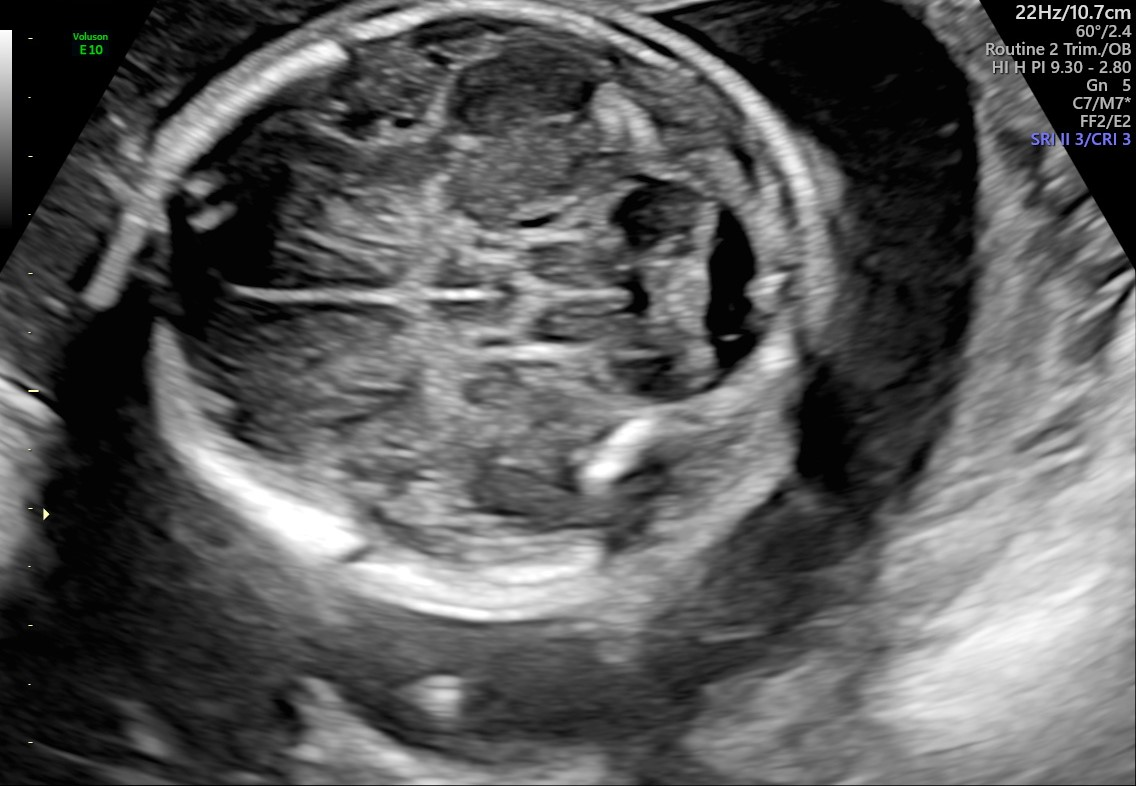
\includegraphics[width= 0.8\textwidth]{img/imagen_cerebelo.jpg} \caption{Ejemplo de ecografía fetal en plano transcerebeloso. Se identifican estructuras anatómicas clave como el vermis cerebeloso, la cisterna magna y los hemisferios cerebelosos.} \label{fig:eco_transcerebeloso} \end{figure} 

A partir de esta necesidad clínica y el avance tecnológico en inteligencia artificial, este proyecto busca desarrollar una herramienta que no solo automatice la segmentación del cerebelo fetal, sino que también facilite su integración en el flujo de trabajo médico habitual. La contribución de este trabajo radica en la propuesta de una solución robusta y escalable, capaz de adaptarse a diversos entornos clínicos y de investigación, sentando las bases para futuras implementaciones en el ámbito del diagnóstico por imagen prenatal. 

De este modo, se pretende contribuir a una atención prenatal más precisa y oportuna, mejorando la calidad del diagnóstico y promoviendo intervenciones tempranas que puedan influir positivamente en el desarrollo neurológico del neonato, siempre teniendo presente que la última palabra en la interpretación diagnóstica corresponde al profesional médico, quien debe evaluar cada caso de forma integral.


\section{Estructura de la memoria}

La memoria se estructura en distintos apartados que recogen tanto los aspectos teóricos como los técnicos y experimentales desarrollados a lo largo del proyecto. Esta organización tiene como objetivo ofrecer una visión clara y progresiva del trabajo realizado, facilitando la comprensión de cada fase del proyecto y su contribución al objetivo global.

\begin{itemize}
    \item \textbf{Introducción}: Contextualiza el problema, resaltando la importancia del análisis del cerebelo fetal en el diagnóstico prenatal y la necesidad de herramientas que mejoren la precisión y eficiencia del proceso. También se incluye una descripción general de la estructura del documento.
    \item \textbf{Objetivos}: Define los objetivos del proyecto, tanto desde el punto de vista técnico como práctico.
    \item \textbf{Conceptos teóricos básicos}: Describe los fundamentos necesarios para entender el proyecto, como los principios del aprendizaje automático y las redes neuronales, así como conceptos relacionados con la anatomía del cerebelo fetal. También se incluye una revisión del estado del arte en segmentación automática aplicada a imágenes médicas.
    \item \textbf{Metodología}: Se detalla el enfoque seguido para el desarrollo del proyecto, incluyendo la estructura del conjunto de datos, el preprocesamiento de imágenes, las técnicas empleadas para el entrenamiento de los modelos y las herramientas utilizadas a lo largo del proceso.
    \item \textbf{Resultados}: Se analizan los modelos entrenados, comparando su rendimiento mediante métricas específicas de segmentación. Se incluyen ejemplos visuales que muestran la segmentación automática en imágenes reales y capturas de la interfaz desarrollada, demostrando su funcionalidad y aplicabilidad práctica.
    \item \textbf{Conclusiones}: Resume los principales hallazgos del proyecto, reflexionando el grado de cumplimiento de los objetivos alcanzados.
    \item \textbf{Líneas futuras de trabajo}: Propone posibles mejoras y ampliaciones que podrían desarrollarse a partir del proyecto actual.
\end{itemize}


\section{Materiales entregados}
Se incorporan a la memoria los anexos, que recogen materiales complementarios que amplían los contenidos desarrollados en el cuerpo principal del trabajo. Los recursos generados a lo largo del proyecto incluyen:
\begin{itemize}
    \item \textbf{Scripts en Python}: código empleado para la preparación del conjunto de datos, el entrenamiento de los modelos de segmentación basados en aprendizaje profundo, las métricas de evaluación y la construcción de una interfaz interactiva para el usuario clínico.
    \item \textbf{Código en LaTeX}: utilizado para la elaboración de la memoria y los anexos.
    \item \textbf{Documentación del proyecto}: incluye tanto la memoria y anexos como otros documentos relevantes, como el proyecto presentado al Comité de ética de Investigación con Medicamentos (CEIM) y las aclaraciones enviadas posteriormente.
    \item \textbf{Resultados}: se recopilan las gráficas y tablas generadas durante la experimentación, que muestran el comportamiento de las arquitecturas evaluadas y sus métricas asociadas.
\end{itemize}

Todo este material se encuentra organizado en el repositorio de GitHub correspondiente al proyecto de segmentación automática del cerebelo fetal, llamado \href{https://github.com/eirarodriguez/fetal_brain_segmentation} {fetal\_brain\_segmentation}.

%\texttt{https://github.com/eirarodriguez/fetal\_brain\_segmentation}.



